%!TEX program = xelatex
\documentclass[10pt, compress, handout]{beamer}
\usepackage[titleprogressbar]{../../cls/beamerthemem}

\setbeamertemplate{caption}[numbered]
\setbeamertemplate{theorems}[numbered]
\newcounter{example}
\resetcounteronoverlays{example}
\newtheorem{crl}{Corollary}[theorem]
\newtheorem{eg}[example]{Example}
\newtheorem*{solution*}{Solution}

\usepackage{booktabs}
\usepackage[scale=2]{ccicons}
\usepackage{minted}

\usepackage{cleveref}
\crefname{example}{Example}{Examples}

\usepgfplotslibrary{dateplot}

\usemintedstyle{trac}

\usepackage{algorithm}
\usepackage[noend]{algpseudocode}
\resetcounteronoverlays{algorithm}

\usepackage{version}
\excludeversion{proof}
\excludeversion{solution*}

\usepackage{mathtools}
\usepackage{multicol}
\usepackage{qtree}

\usepackage{tikz}

\makeatletter
\def\old@comma{,}
\catcode`\,=13
\def,{%
    \ifmmode%
    \old@comma\discretionary{}{}{}%
    \else%
    \old@comma%
    \fi%
}
\makeatother

\title{CSCI 3190 Tutorial of Week 11}
\subtitle{Longest Common Subsequence}
\author{LI Haocheng}
\institute{Department of Computer Science and Engineering}

\begin{document}

\maketitle

\begin{frame}[allowframebreaks]
\frametitle{Longest Common Subsequence}
\begin{eg}
    \begin{enumerate}[(a)]
        \item Find the longest common subsequence between $\alpha = \mathtt{abcbdaccdb}$ and $\beta = \mathtt{bbcad}$ by constructing a table $len$ where $len[i, j]$ is the length of the longest common subsequence between $\alpha[1]\alpha[2]\cdots\alpha[i]$ and $\beta[1]\beta[2]\cdots\beta[j]$ where $i = 1\cdots 10$ and $j = 1\cdots 5$.
        \item From the table $len$, find all the longest common subsequences between $\alpha$ and $\beta$. For each of the longest common subsequences, show how it can be found from the table.
    \end{enumerate}
\end{eg}
\newpage
\begin{solution*}
    \begin{table}
        \centering
        \caption{The Table $len$}
        \label{t-6}
        \begin{tabular}{c|ccccccccccc}
            \toprule 
            & 0 & a & b & c & b & d & a & c & c & d & b \\ 
            \midrule 
            0 & 0 & 0 & 0 & 0 & 0 & 0 & 0 & 0 & 0 & 0 & 0 \\ 
            b & 0 & 0 & \alert{1} & 1 & 1 & 1 & 1 & 1 & 1 & 1 & 1 \\ 
            b & 0 & 0 & 1 & 1 & \alert{2} & 2 & 2 & 2 & 2 & 2 & 2 \\ 
            c & 0 & 0 & 1 & \alert{2} & 2 & 2 & 2 & \alert{3} & 3 & 3 & 3 \\ 
            a & 0 & 1 & 1 & 2 & 2 & 2 & \alert{3} & 3 & 3 & 3 & 3 \\ 
            d & 0 & 1 & 1 & 2 & 2 & 3 & 3 & 3 & 3 & \alert{4} & 4 \\ 
            \bottomrule 
        \end{tabular}
    \end{table}
\end{solution*}
\end{frame}

\begin{frame}[allowframebreaks]
\frametitle{Recursive Algorithm}
\begin{eg}
    Consider the longest common subsequence problem between sequence $A[1\cdots m]$ and sequence $B[1\cdots n]$. Give a
    recursive algorithm to print out ALL the longest common subsequences assuming that you already build the
    table $T[1\cdots m, 1\cdots n]$ where the entry $T[j, k]$ represents the length of the longest common subsequence between $A[1\cdots j]$ and $B[1\cdots k]$.
\end{eg}
\begin{solution*}
    See Algorithm \ref{a-5}.
    \begin{algorithm}[H]
        \caption{Print Out ALL the LCSes}
        \label{a-5}
        \begin{algorithmic}
            \Procedure{All}{$T$, $A$, $B$, $j$, $k$}
            \If{$j \cdot k = 0$} \Return $\{``"\}$
            \ElsIf{$A[j] = B[k]$} \Return $\{C + A[j] \colon Z \in \Call{All}{T, A, B, j - 1, k - 1}\}$
            \Else
            \State $R \coloneqq \{\}$
            \If{$T[j, k - 1] \ge T[j - 1, k]$} $R \coloneqq R \cup \Call{All}{T, A, B, j, k - 1}$
            \EndIf
            \If{$T[j - 1, k] \ge T[j, k - 1]$} $R \coloneqq R \cup \Call{All}{T, A, B, j - 1, k}$
            \EndIf
            \State \Return $R$
            \EndIf
            \EndProcedure
        \end{algorithmic}
    \end{algorithm}
\end{solution*}
\end{frame}

\begin{frame}[fragile]
\frametitle{Euler Path}
\onslide<1->\begin{columns}
    \begin{column}{.5\linewidth}
        \begin{eg}
            Determine whether the given graph has an
            Euler circuit. Construct such a circuit when one exists. If
            no Euler circuit exists, determine whether the graph has an
            Euler path and construct such a path if one exists.
        \end{eg}
    \end{column}
    \begin{column}{.5\linewidth}
        \begin{figure}
            \centering
            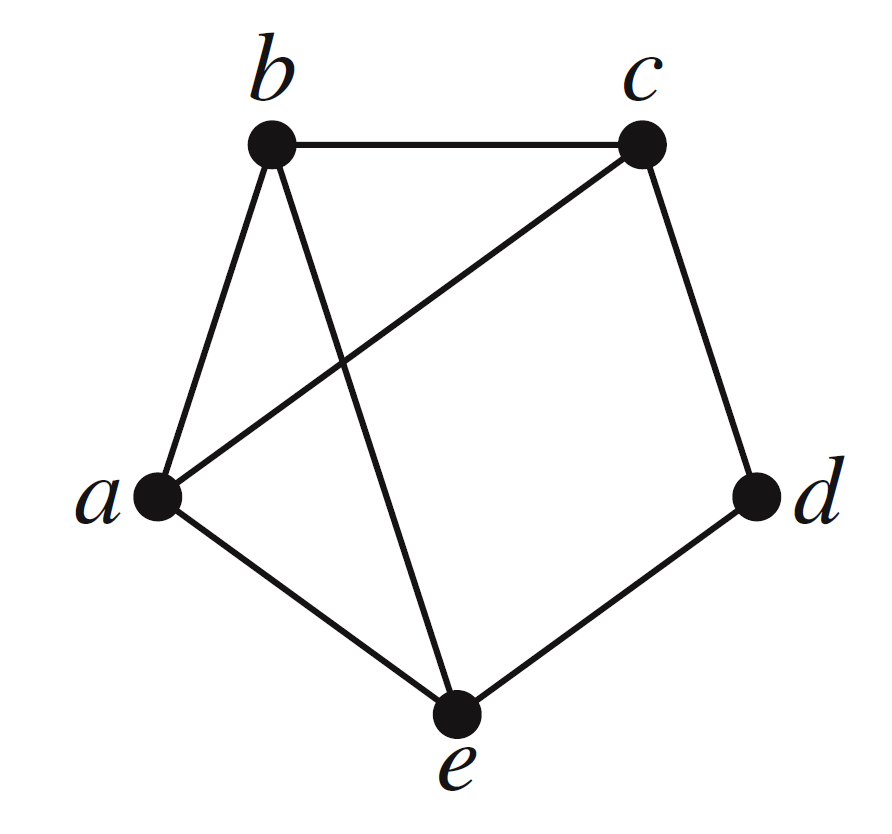
\includegraphics[width=.6\linewidth]{f-10-5-e-1}
        \end{figure}
    \end{column}
\end{columns}
\onslide<2>\begin{solution*}
    Neither.
\end{solution*}
\end{frame}

\begin{frame}[fragile]
\frametitle{Euler Circuit}
\onslide<1->\begin{columns}
    \begin{column}{.5\linewidth}
        \begin{eg}
            Determine whether the given graph has an
            Euler circuit. Construct such a circuit when one exists. If
            no Euler circuit exists, determine whether the graph has an
            Euler path and construct such a path if one exists.
        \end{eg}
    \end{column}
    \begin{column}{.5\linewidth}
        \begin{figure}
            \centering
            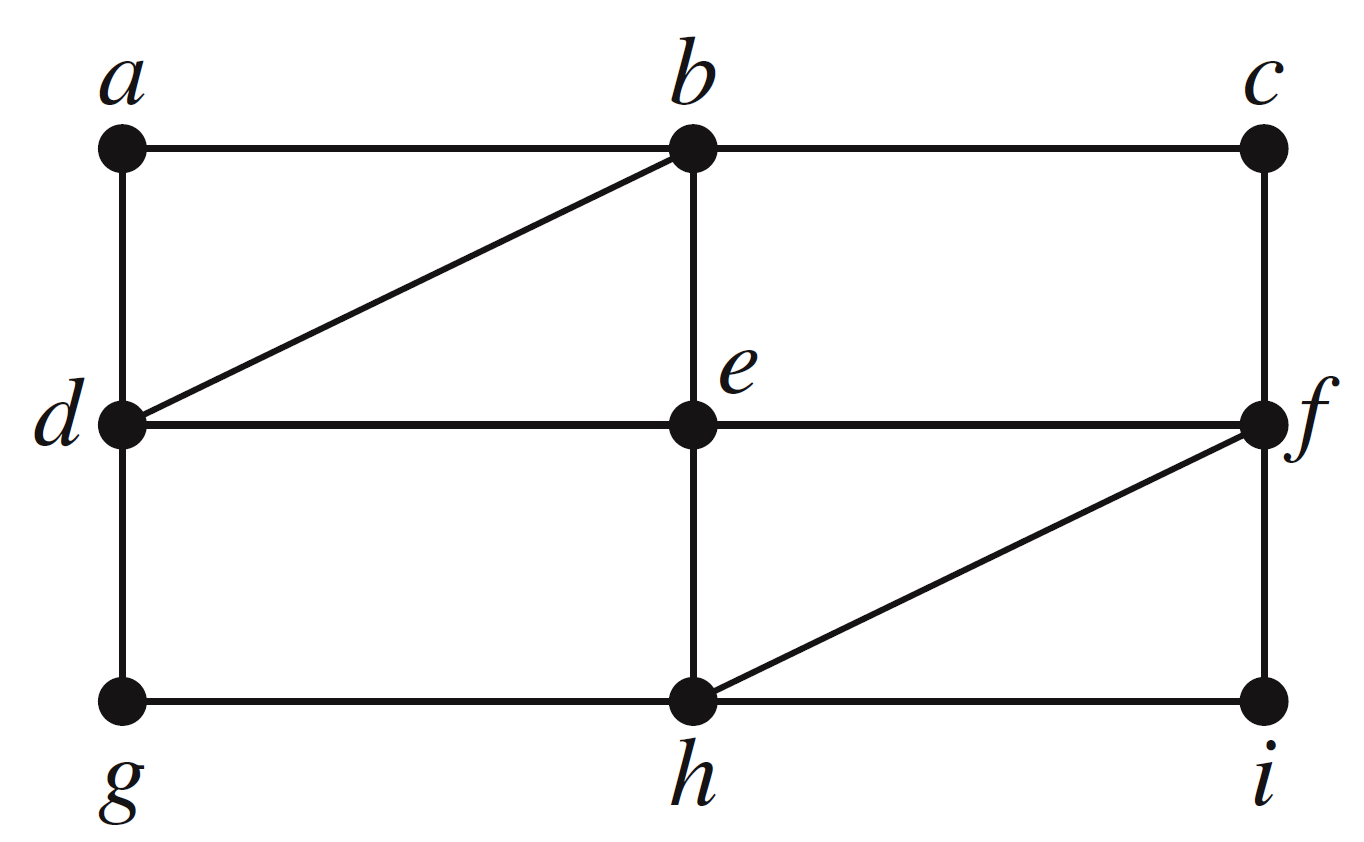
\includegraphics[width=.8\linewidth]{f-10-5-e-2}
        \end{figure}
    \end{column}
\end{columns}
\onslide<2>\begin{solution*}
    $a, b, c, f, e, b, d, e, h, f, i, h, g, d, a.$
\end{solution*}
\end{frame}

\begin{frame}[fragile]
\frametitle{Hamilton Path}
\onslide<1->\begin{columns}
    \begin{column}{.5\linewidth}
        \begin{eg}
            Which of the simple graphs in Figure have a Hamilton circuit or, if not, a Hamilton path?
        \end{eg}
    \end{column}
    \begin{column}{.5\linewidth}
        \begin{figure}
            \centering
            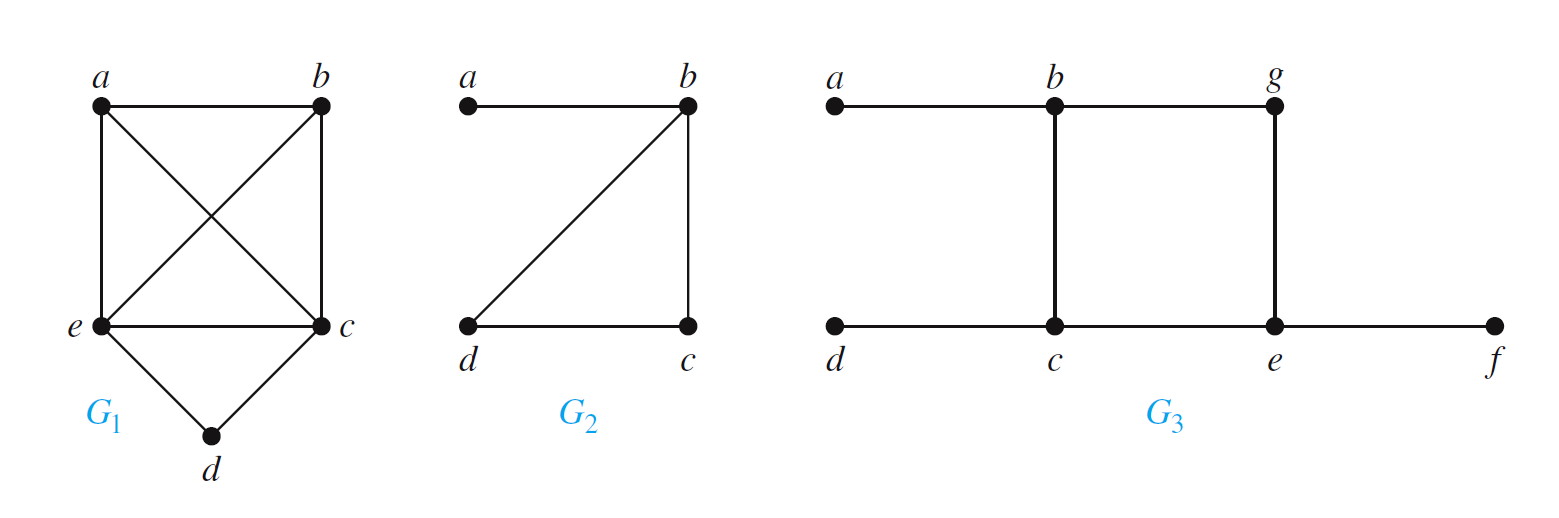
\includegraphics[width=\linewidth]{f-10-5-10}
        \end{figure}
    \end{column}
\end{columns}
\onslide<2>\begin{solution*}
    $G_1$ has a Hamilton circuit: $a, b, c, d, e, a$. There is no Hamilton circuit in $G_2$ (this can
    be seen by noting that any circuit containing every vertex must contain the edge $\{a, b\}$ twice),
    but $G_2$ does have a Hamilton path, namely, $a, b, c, d$. $G_3$ has neither a Hamilton circuit nor a
    Hamilton path, because any path containing all vertices must contain one of the edges $\{a, b\}, \{e, f\}$, and $\{c, d\}$ more than once.
\end{solution*}
\end{frame}

\begin{frame}[fragile]
\frametitle{Hamilton Circuit}
\onslide<1->\begin{columns}
    \begin{column}{.5\linewidth}
        \begin{eg}
            Show that neither graph displayed in Figure has a Hamilton circuit.
        \end{eg}
    \end{column}
    \begin{column}{.5\linewidth}
        \begin{figure}
            \centering
            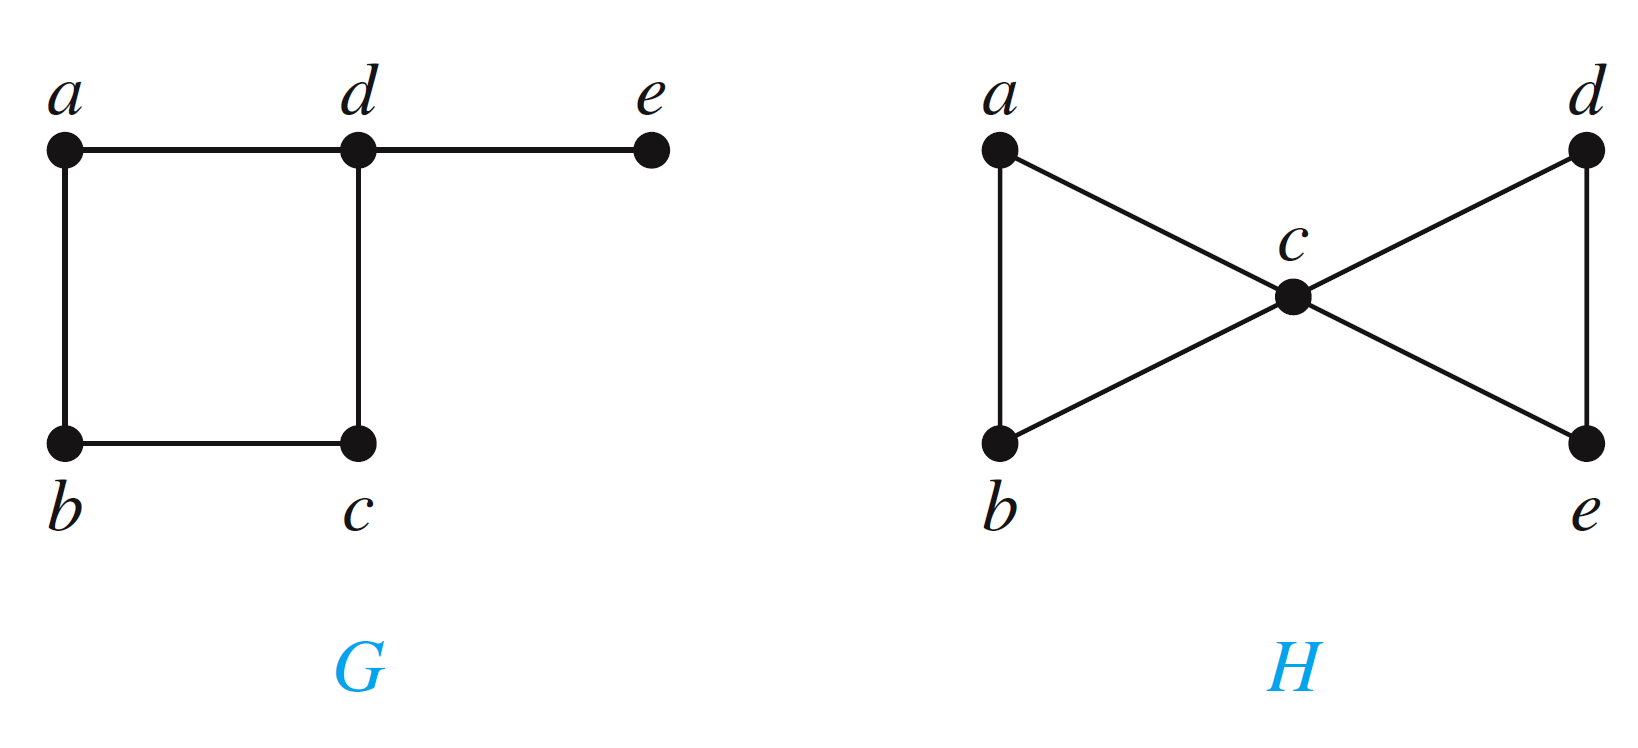
\includegraphics[width=\linewidth]{f-10-5-11}
        \end{figure}
    \end{column}
\end{columns}
\onslide<2>\begin{solution*}
    There is no Hamilton circuit in $G$ because $G$ has a vertex of degree one, namely, $e$. Now consider $H$. Because the degrees of the vertices $a, b, d$, and $e$ are all two, every edge incident with these vertices must be part of any Hamilton circuit. It is now easy to see that no Hamilton circuit can exist in $H$, for any Hamilton circuit would have to contain four edges incident with c, which is impossible.
\end{solution*}
\end{frame}

\begin{frame}[fragile]
\frametitle{Shortest Path}
\onslide<1->\begin{columns}
    \begin{column}{.5\linewidth}
        \begin{eg}
            Find the length of a shortest path between $a$
            and $z$ in the given weighted graph.
        \end{eg}
    \end{column}
    \begin{column}{.5\linewidth}
        \begin{figure}
            \centering
            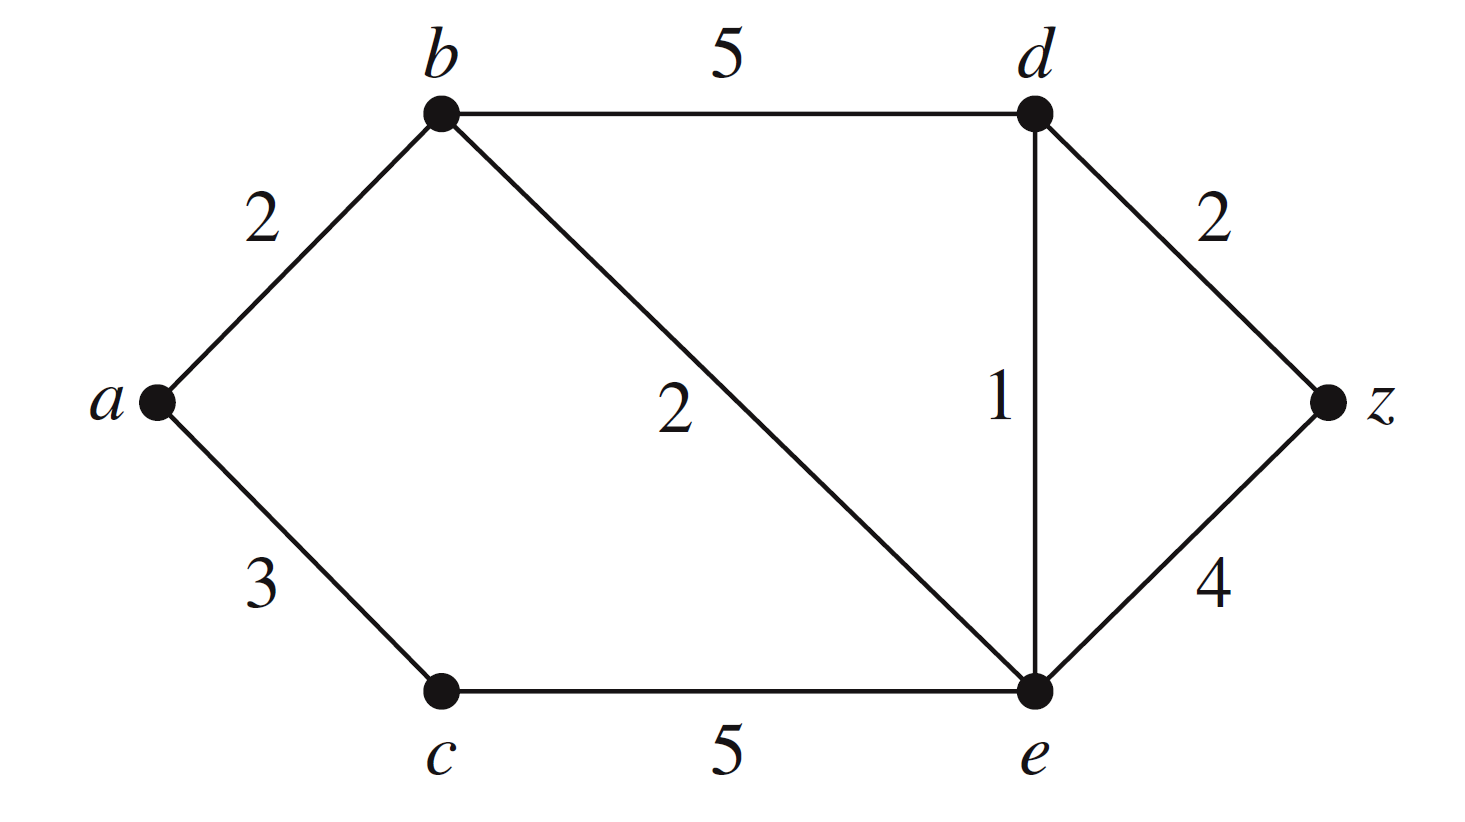
\includegraphics[width=\linewidth]{f-10-6-e-2}
        \end{figure}
    \end{column}
\end{columns}
\onslide<2>\begin{solution*}
    \begin{equation}
    2 + 2 + 1 + 2 = 7.
    \end{equation}
\end{solution*}
\end{frame}

\plain{Questions?}

\end{document}
